% \DocumentMetadata 在文档类之前声明输出元数据；pdfversion=1.5 固定 PDF 版本，lang=zh-CN 标记主要语言为中文。
\DocumentMetadata{pdfversion=1.5,lang=zh-CN}

% standalone 文档类会按图形边界裁切页面；tikz 选项加载绘图支持，border=10pt 在图形四周保留 10 磅空白。
\documentclass[tikz,border=10pt]{standalone}
% CJK 宏包处理后面节点中的中文字符，tikz 宏包提供 tikzpicture、node、draw 等绘图命令。
\usepackage{CJK}
\usepackage{tikz}

% \usetikzlibrary 一次加载两个 TikZ 库：arrows.meta 提供 Latex 箭头尖，positioning 提供 right=of 等相对定位语法。
\usetikzlibrary{arrows.meta,positioning}

\begin{document}
\begin{CJK*}{UTF8}{gbsn}
% \newcommand 把两个中文词封装为可复用命令；每个 \CJKchar 用十六进制编码指定一个汉字，调用时无需重复长写法。
\newcommand{\sourcesuffix}{\CJKchar[UTF8]{"6E}{"90}\CJKchar[UTF8]{"78}{"01}}
\newcommand{\outputsuffix}{\CJKchar[UTF8]{"8F}{"93}\CJKchar[UTF8]{"51}{"FA}}
% tikzpicture 的方括号设置全图参数：node distance 控制节点间距，box/.style 定义节点外观，arrow/.style 定义线条和箭头尖。
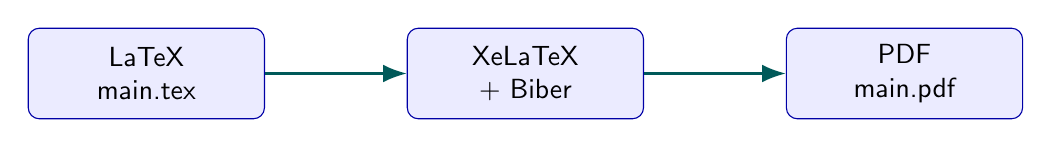
\begin{tikzpicture}[
    node distance=1.8cm,
    box/.style={
        draw=blue!65!black,
        fill=blue!8,
        rounded corners,
        minimum width=3.0cm,
        minimum height=1.15cm,
        align=center,
        font=\sffamily
    },
    arrow/.style={-{Latex[length=3mm]},thick,draw=teal!70!black}
]
    % \node[样式] (名称) {内容} 创建可引用节点；right=of 让后一个节点依次放在前一个节点右侧。
    \node[box] (source) {LaTeX \sourcesuffix\\main.tex};
    \node[box,right=of source] (engine) {XeLaTeX\\+ Biber};
    \node[box,right=of engine] (pdf) {PDF \outputsuffix\\main.pdf};

    % \draw[arrow] (起点) -- (终点) 按预设 arrow 样式连接节点，形成从源码到工具再到 PDF 的流程。
    \draw[arrow] (source) -- (engine);
    \draw[arrow] (engine) -- (pdf);
\end{tikzpicture}
\end{CJK*}
\end{document}
